\documentclass[]{article}
\usepackage{lmodern}
\usepackage{amssymb,amsmath}
\usepackage{ifxetex,ifluatex}
\usepackage{fixltx2e} % provides \textsubscript
\ifnum 0\ifxetex 1\fi\ifluatex 1\fi=0 % if pdftex
  \usepackage[T1]{fontenc}
  \usepackage[utf8]{inputenc}
\else % if luatex or xelatex
  \ifxetex
    \usepackage{mathspec}
  \else
    \usepackage{fontspec}
  \fi
  \defaultfontfeatures{Ligatures=TeX,Scale=MatchLowercase}
\fi
% use upquote if available, for straight quotes in verbatim environments
\IfFileExists{upquote.sty}{\usepackage{upquote}}{}
% use microtype if available
\IfFileExists{microtype.sty}{%
\usepackage[]{microtype}
\UseMicrotypeSet[protrusion]{basicmath} % disable protrusion for tt fonts
}{}
\PassOptionsToPackage{hyphens}{url} % url is loaded by hyperref
\usepackage[unicode=true]{hyperref}
\hypersetup{
            pdftitle={Analytics},
            pdfauthor={Silke Meiner, Rafaela Neff},
            pdfborder={0 0 0},
            breaklinks=true}
\urlstyle{same}  % don't use monospace font for urls
\usepackage[margin=1in]{geometry}
\usepackage{natbib}
\bibliographystyle{plainnat}
\usepackage{graphicx,grffile}
\makeatletter
\def\maxwidth{\ifdim\Gin@nat@width>\linewidth\linewidth\else\Gin@nat@width\fi}
\def\maxheight{\ifdim\Gin@nat@height>\textheight\textheight\else\Gin@nat@height\fi}
\makeatother
% Scale images if necessary, so that they will not overflow the page
% margins by default, and it is still possible to overwrite the defaults
% using explicit options in \includegraphics[width, height, ...]{}
\setkeys{Gin}{width=\maxwidth,height=\maxheight,keepaspectratio}
\IfFileExists{parskip.sty}{%
\usepackage{parskip}
}{% else
\setlength{\parindent}{0pt}
\setlength{\parskip}{6pt plus 2pt minus 1pt}
}
\setlength{\emergencystretch}{3em}  % prevent overfull lines
\providecommand{\tightlist}{%
  \setlength{\itemsep}{0pt}\setlength{\parskip}{0pt}}
\setcounter{secnumdepth}{0}
% Redefines (sub)paragraphs to behave more like sections
\ifx\paragraph\undefined\else
\let\oldparagraph\paragraph
\renewcommand{\paragraph}[1]{\oldparagraph{#1}\mbox{}}
\fi
\ifx\subparagraph\undefined\else
\let\oldsubparagraph\subparagraph
\renewcommand{\subparagraph}[1]{\oldsubparagraph{#1}\mbox{}}
\fi

% set default figure placement to htbp
\makeatletter
\def\fps@figure{htbp}
\makeatother


\title{Analytics}
\author{Silke Meiner, Rafaela Neff}
\date{10 3 2021}

\begin{document}
\maketitle

{
\setcounter{tocdepth}{2}
\tableofcontents
}
\section{Abstract}\label{abstract}

We present and compare machine learnt classification algorithms for
diagnosing breast tumor cells as benign or malignant. The algorithms
were trained on tabular data consisting of features extracted from
microscopic images of fine-needle aspirates / biopsies.

We get reasonably good results from Logistic regression and were able to
improve these results through single and multi-layer neural networks.
The final neural network with an accuracy of \ldots{}, sensitivity of
\ldots{} and specificity \ldots{} is being audited at the German
Gesundheitsministerium to become a state approved diagnostic tool.

\section{Business Understanding}\label{business-understanding}

Breast cancer is the most common cancer for women and ranks highest for
cancer-related deaths in women in Germany: In 2016 there were 68,950
women and 710 men suffering from Breast Cancer (ICD-10 C50). In 2020
18,570 women and 1 men have died of breast cancer.

The situation is similar in many other countries.

Tumors can build in the human body as some cells grow more than they
normally should. If this growth is not limiting itself and destroys body
tissue and hinders body functions the tumor is labeled malignant and
called cancer.

Tumors are classified in a binary fashion as either malignant or benign.
Their difference in microscopic imagery are shown in figure
\ref{fig:normal-vs-cancer}. A typical first step when diagnosing a tumor
is to do a fine needle aspirate (FNA) of a breast mass and looking at
the cells through a microscope, describing characteristics of the cell
nuclei. Further treatment differs according to the tumor diagnosis as
benign or malignant.

\begin{figure}
    \centering
    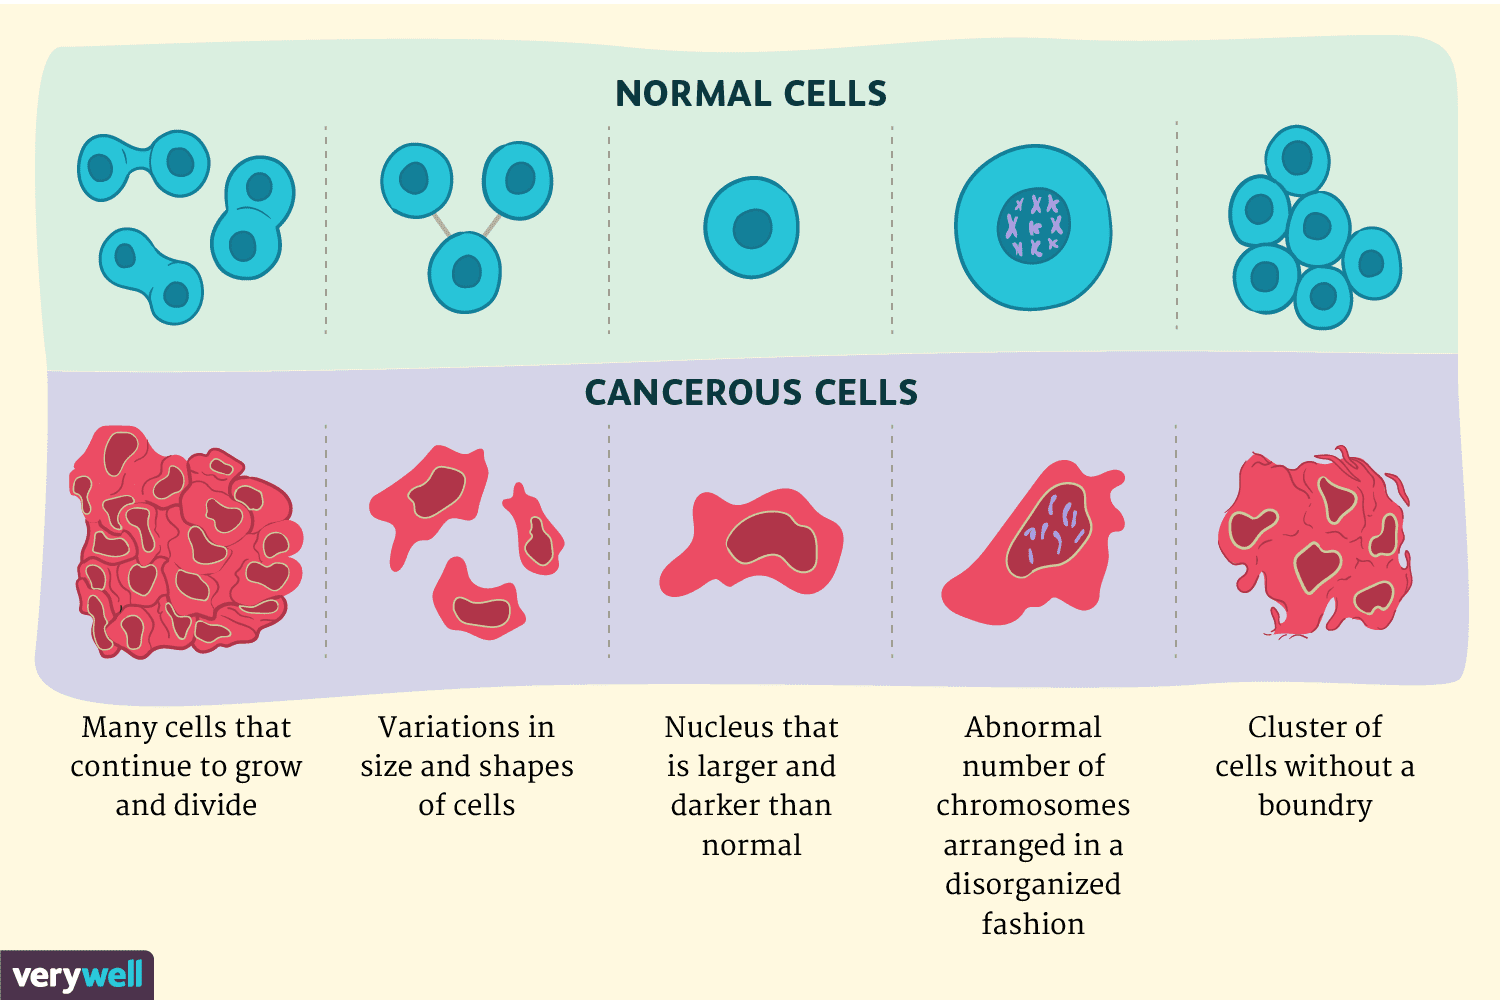
\includegraphics[width=0.8\textwidth]{images/normal-vs-cancerous-cells.png}
    \caption{benign / normal and malignant / cancerous  cells}
    \label{fig:normal-vs-cancer}
\end{figure}

Sources :

\begin{itemize}
\item
  \cite{rki}
\item
  \cite{malignant-and-benign}
\item
  \cite{cancer-cells-vs-normal}
\end{itemize}

\section{Data Sources and Data
Understanding}\label{data-sources-and-data-understanding}

The data for this project was collected in 1995 by the University of
Wisconsin and made available to us through Prof.~Dr.~Nick Street of the
University of Iowa.

The data can be downloaded from the University of California, Irvine,
\url{https://archive.ics.uci.edu/ml/datasets/Breast+Cancer+Wisconsin+\%28Diagnostic\%29}

\subsection{Data Understanding}\label{data-understanding}

Our data set is mid sized with 569 observations for 30 numeric feature
variables. Each observation has an additional binary diagnosis as benign
or malignant. The data set is slightly unbalanced with 357 (63\%) being
benign and 212 (37\%) malignant cases. We made malignant the positive
class.

Some predictor variables are highly correlated.

When there is correlation of feature variables with the target variable,
it is mostly positive and not exceeding \ldots{}

\subsection{Data Visualisation, looped back after first
modelling}\label{data-visualisation-looped-back-after-first-modelling}

This visualisation of our data ba application of PCA was developed after
a first loop in the CRISP model. In sequential reading this serves as a
general visualisation now and will become important later on.

** put images A.png and B.png here **

\begin{figure}
    \centering
    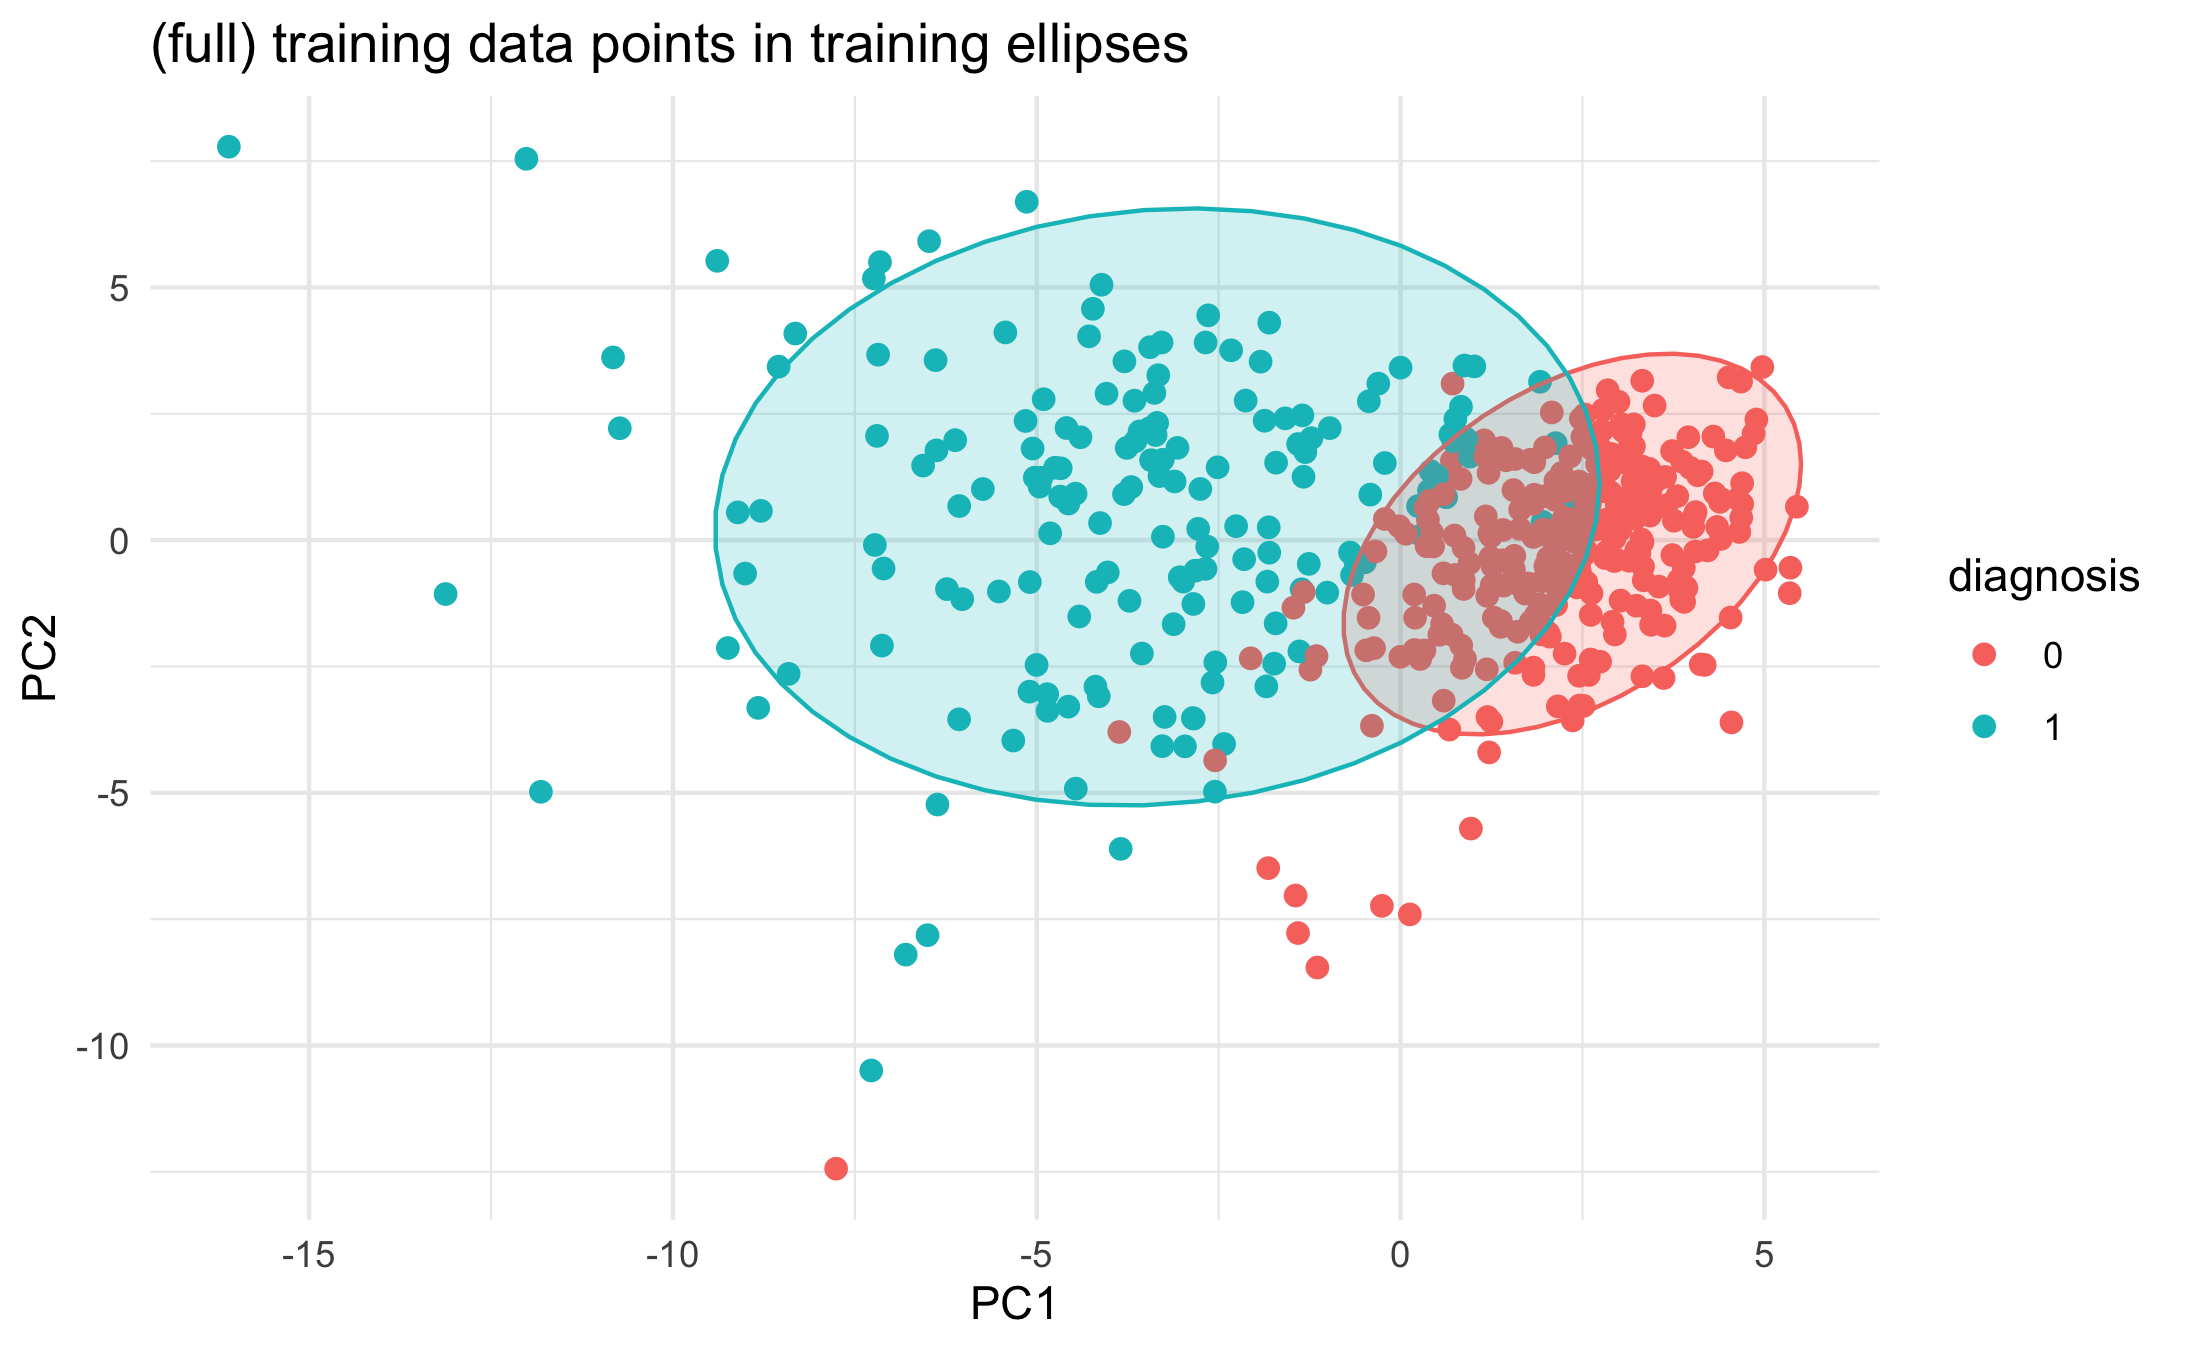
\includegraphics[width=0.8\textwidth]{images/A-training-full-PCA.png}
    \caption{Caption A-training-full-PCA.png}
    \label{fig:A-training-full-PCA}
\end{figure}

\begin{figure}
    \centering
    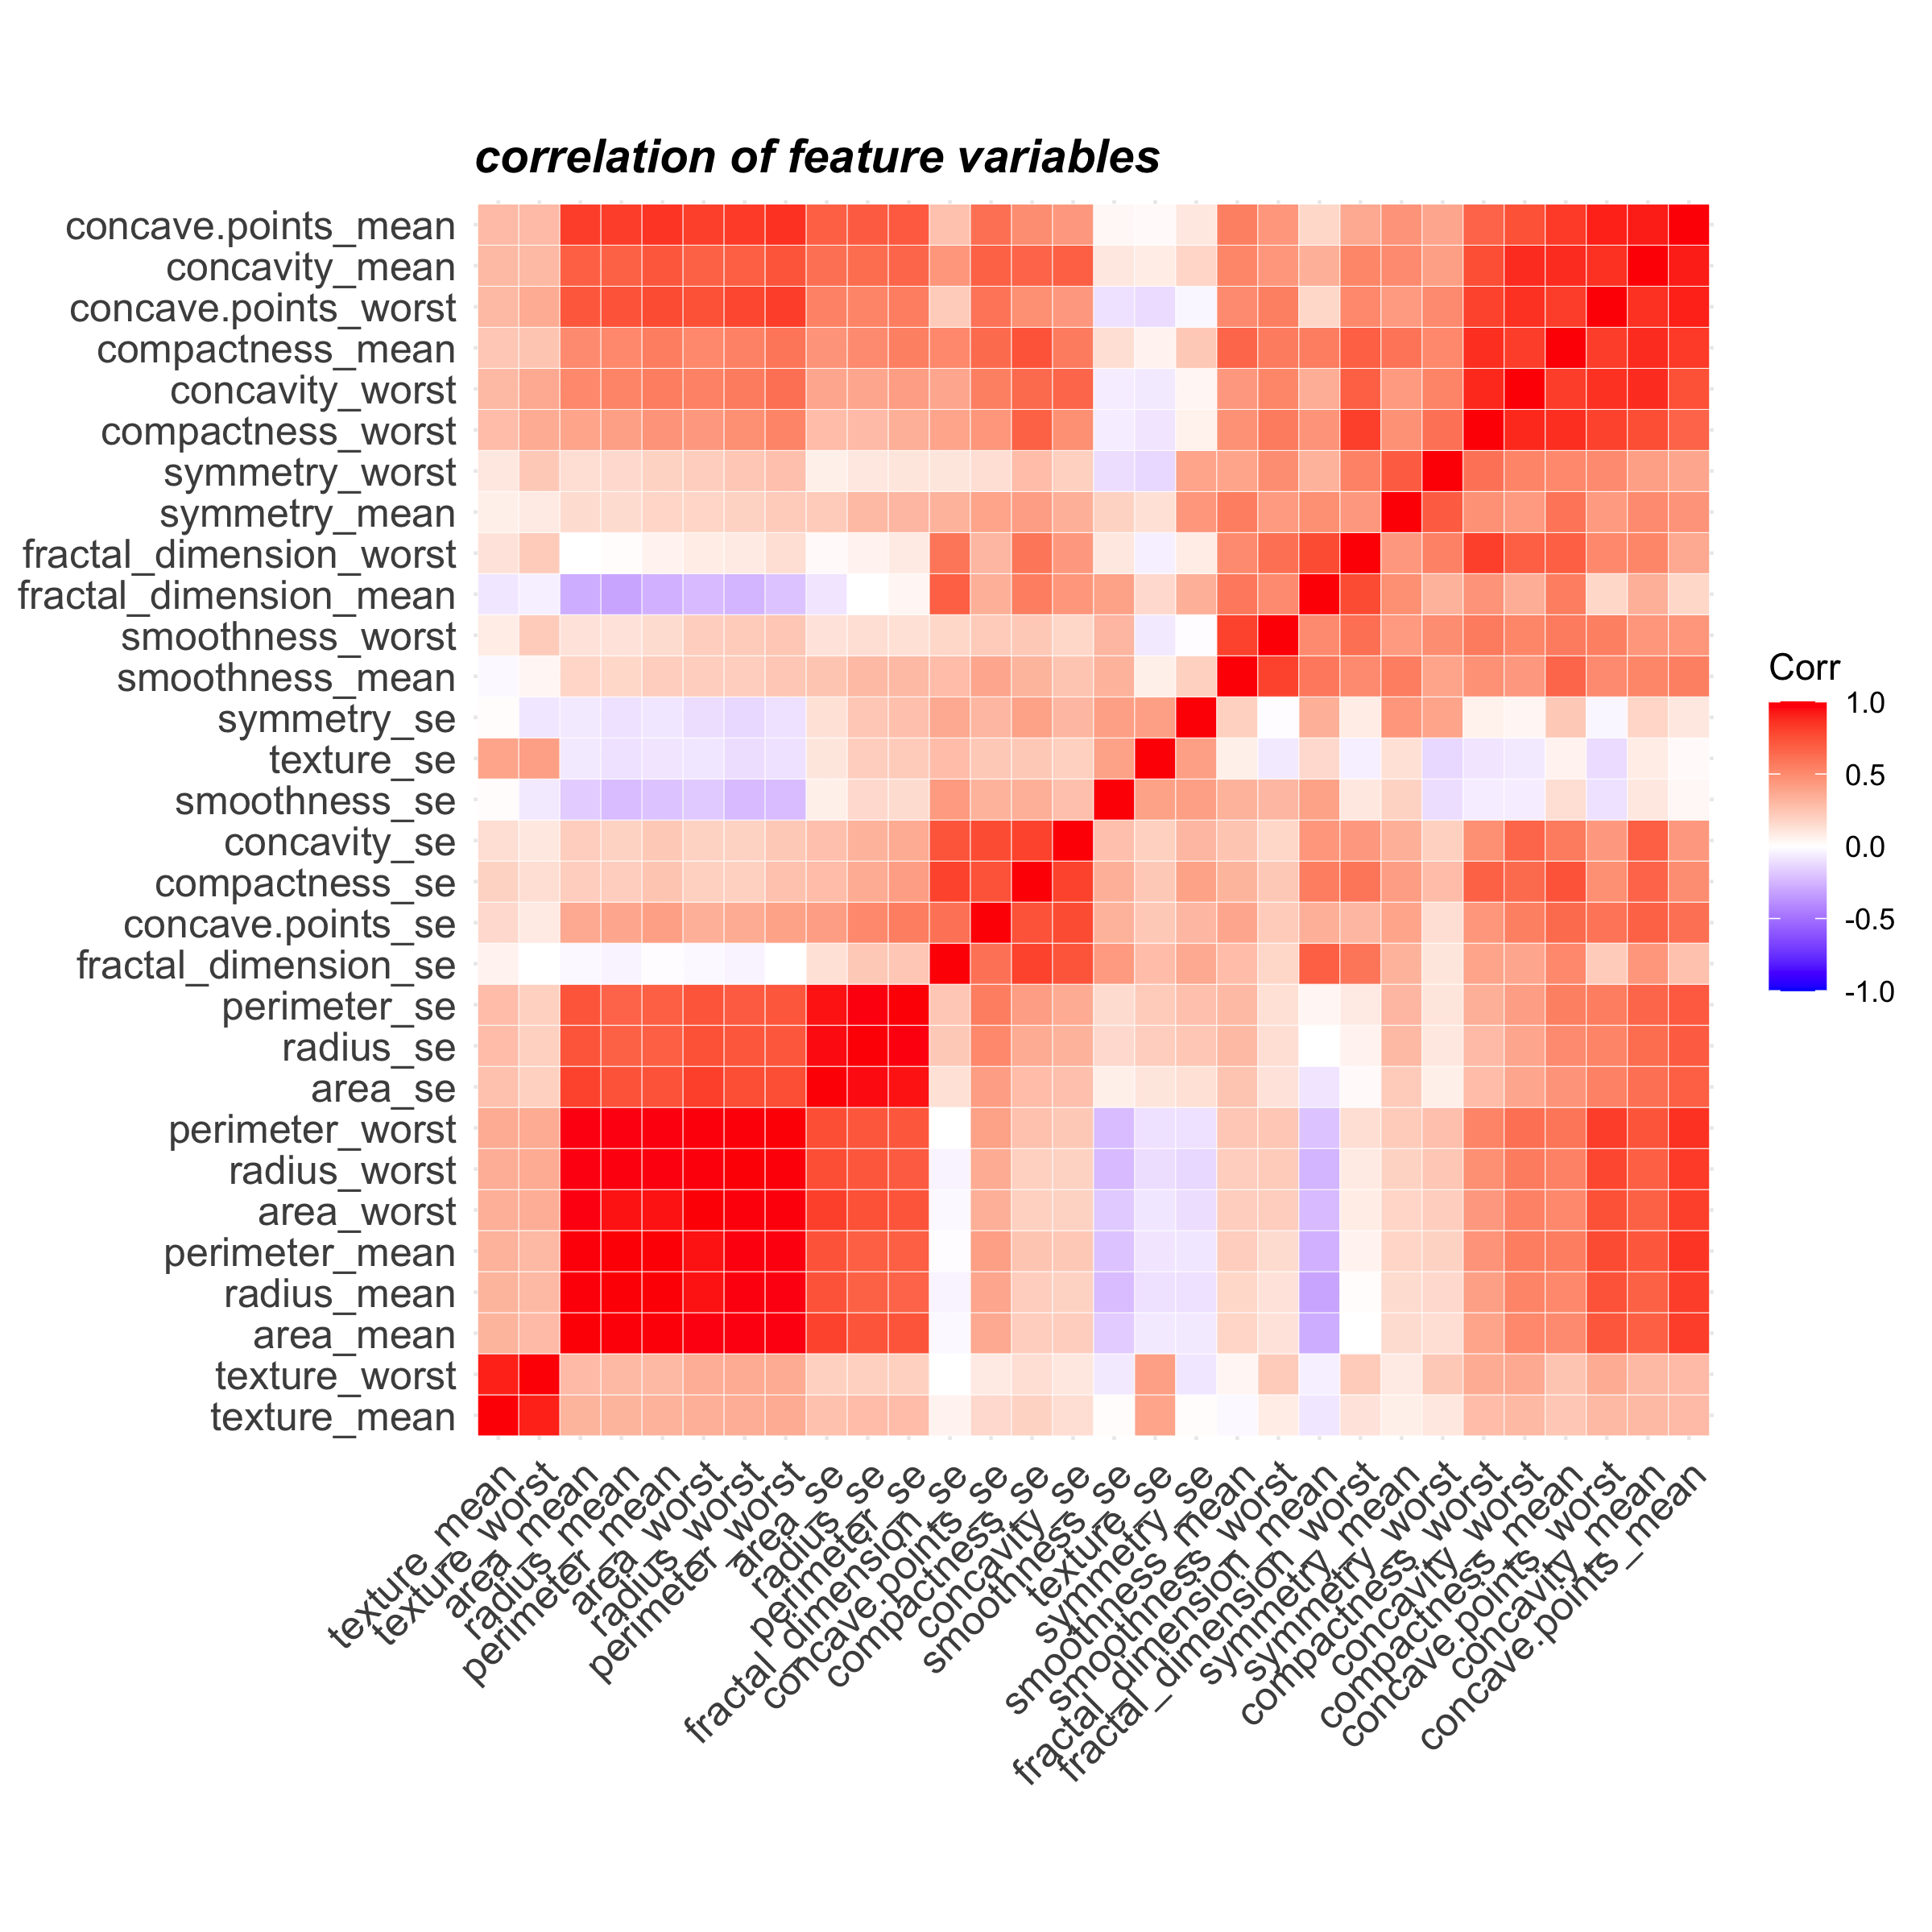
\includegraphics[width=0.8\textwidth]{images/correlation-features.png}
    \caption{Caption correlation-features.png}
    \label{fig:correlation-feature}
\end{figure}

\section{Data Preparation}\label{data-preparation}

Since there were no missing data in our set we did not impute anything.
Data was used as delivered.

Data was separated into training and test sets, each with a separate
file. The data was split 80/20 and with stratification wrt to the
diagnosis.

For further details, please look into our notebook on data preparation.

\section{Modeling}\label{modeling}

To solve the classification task we applied two machine learning
methods: Logistic regression and neural networks.

In classification tasks we generally have predictor variables and a
target variable. In binary classification the target variable can take
one of two distinct values, interpreted as the two classes on option.

The methodological (?) similarities of both machine learning models are
in the training and evaluation of the model. The training requires a
training set of observed data points including the true values of the
target variable. For evaluation a test set of observed data points
including the true values of the target variable is required. Training
and test set need to be disjoint. On the test set the algorithm predicts
classes for the data points and predictions are compared with the
targets. Counting correct and not correct classifications and setting
them in relation results in accuracy, sensitivity and specificity as
measures of success.

\subsection{Logistic Regression}\label{logistic-regression}

Given: Some numeric data, in tabular form of \(n\) rows and \(p+1\)
variables. \(p\) variables are predictors and the remaining variable is
the target. The target takes one of two values, interpreted as two
classes, with one class defined as the positive class.

Desired: The class the data point belongs to with a probability
distribution over the two classes (stating the probabilities that the
data point belongs to each class).

Linear regression uses a linear combination of the variables to predict
another numeric target variable. logistic regression does linear
regression for the log-odds of the desired probabilities.

\[
{log-odds} = \beta_0 + \beta_1 x_1 + \dots + \beta_p x_p     
\]

The log-odds are transformed into (conditional) probabilities for the
positive class through the logistic function \[  \sigma(.)  \],
sometimes called sigmoid.

\[
p(\bf{x}) = \sigma(\text{log-odds}) = \sigma(\beta_0 + \beta_1 x_1 + \dots + \beta_p x_p ) 
\]

with
\[ \bf{x}= ( x_1, \dots, x_p) , p(\bf{x}) = \mathbf{P}\left(\text{target = positive class} | \text{predictors } = \bf{x} \right) \]
and \[ \sigma(a) = \frac{1}{1+e^{-a}} \].

If the probability for the positive class \[ p(\bf{x})\] exceeds a
threshold, the data point is classified as the positive class.

The performance of the model is determined by its coefficients / weights
\[\beta \]. Finding the best / suitable coefficients is done in
training. For logistic regression there are several training methods
performed by statistical software like R.

In the beginning of running a logistic regression we ran into a
`problem' hinting to perfect separation of classes in our data set. We
decided to ignore the problem and try to get the best possible results
from logistic regression. Another option would have been: change to
support vector machines which could directly exploit the seperability in
our data.

Sources:

Log Regression (\cite{logreg})

for ignoring the problem of complete separation (\cite{ucla})

Finding coefficients for logistic regression: (\cite{newton})

\subsection{Artificial Neural
Networks}\label{artificial-neural-networks}

\subsubsection{Model overview}\label{model-overview}

Artificial Neural Networks are forecasting methods based on simple
mathematical models of the brain. They allow complex nonlinear
relationships between the response variable and its predictors.
(\cite{otexts})

\begin{figure}
    \centering
    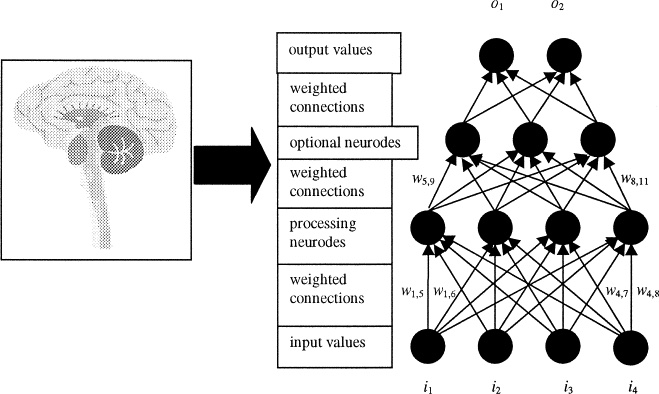
\includegraphics[width=0.8\textwidth]{images/ann.jpg}
    \caption{Sample artificial neural network architecture (not all weights are shown) - (\cite{ann})}
    \label{fig:ann}
\end{figure}

Connections between neurons are weighted to represent the connection
strength. It's the artificial pendant of the synapses in the brain.
Positive weights are used to excite neurons in the network and negative
weights are used to inhibit other neurons.

\textbf{Architecture}: Topology of the network

\textbf{Activities}: How do ANNs Neurons respond to one another to
produce a certain behavior.

\textbf{Learning Rule}: How should weights and connections change
regarding the input, output, and error-rate.

\textbf{Deep Neural Network}: Network with many hidden layers.

ANN structure can be described as its Architecture, Activities, and
Learning Rule.

\subsubsection{Implementation}\label{implementation}

We've implemented two different kinds of Neural Network. One wth R's
nnet-Package (\cite{nnet}) and one using the R-Package for h2o
(\cite{h2o}).

Nnet is supporting one hidden layer only and comes with poor
explainability. Since the results on the test-data were poor showing an
accuracy below 90\% we've choosen h2o over nnet and will evaluate
further on h2o throughout this report.

\subsection{Normalization}\label{normalization}

Depending on the implementation and the specific model different
standardization is used throughout this project in order to ensure that
all features have the same chance of importance fitting the model.

The nnet Implementation uses it's own user-defined-function (UDF)
standardizing via min-max-normalization using this formular: \[
\frac{x_i-\min(x_i)}{\max(x_i)-\min(x_i)}
\]

The h2o-Implementation uses the Standard Deviation implicitly,
standardazing via \[
\frac{x-mean}{stddev}
\]

\subsubsection{Proposed Model
architecture}\label{proposed-model-architecture}

We arrived at the selected Hyperparameters by performing a grid-search.

\textbf{hidden\_dropout\_ratios}: (Activation type:
\textbf{RectifierWithDropout}) Specify the hidden layer dropout ratio to
improve generalization. Specify one value per hidden layer. The range is
\textgreater{}= 0 to \textless{}1, and the default is 0.5.

The amount of dropout on the input layer can be specified for all
activation functions, but hidden layer dropout is only supported is set
to WithDropout. The default hidden dropout is 50\%, so you don't need to
specify anything but the activation type to get good results, but you
can set the hidden dropout values for each layer separately.

Performing a grid-search we've chosen the model with the highest
auc-value which isn't 1. This decision is based on preventing
overfitting. The False-Negatives were examined manually to get a grip on
the real-world-value of our model. What we are trying to prevent is our
model telling that a person doesn't have breast-cancer, when in fact he
or she does.

Considering all this we did arrive at the following architecture:

\begin{figure}
    \centering
    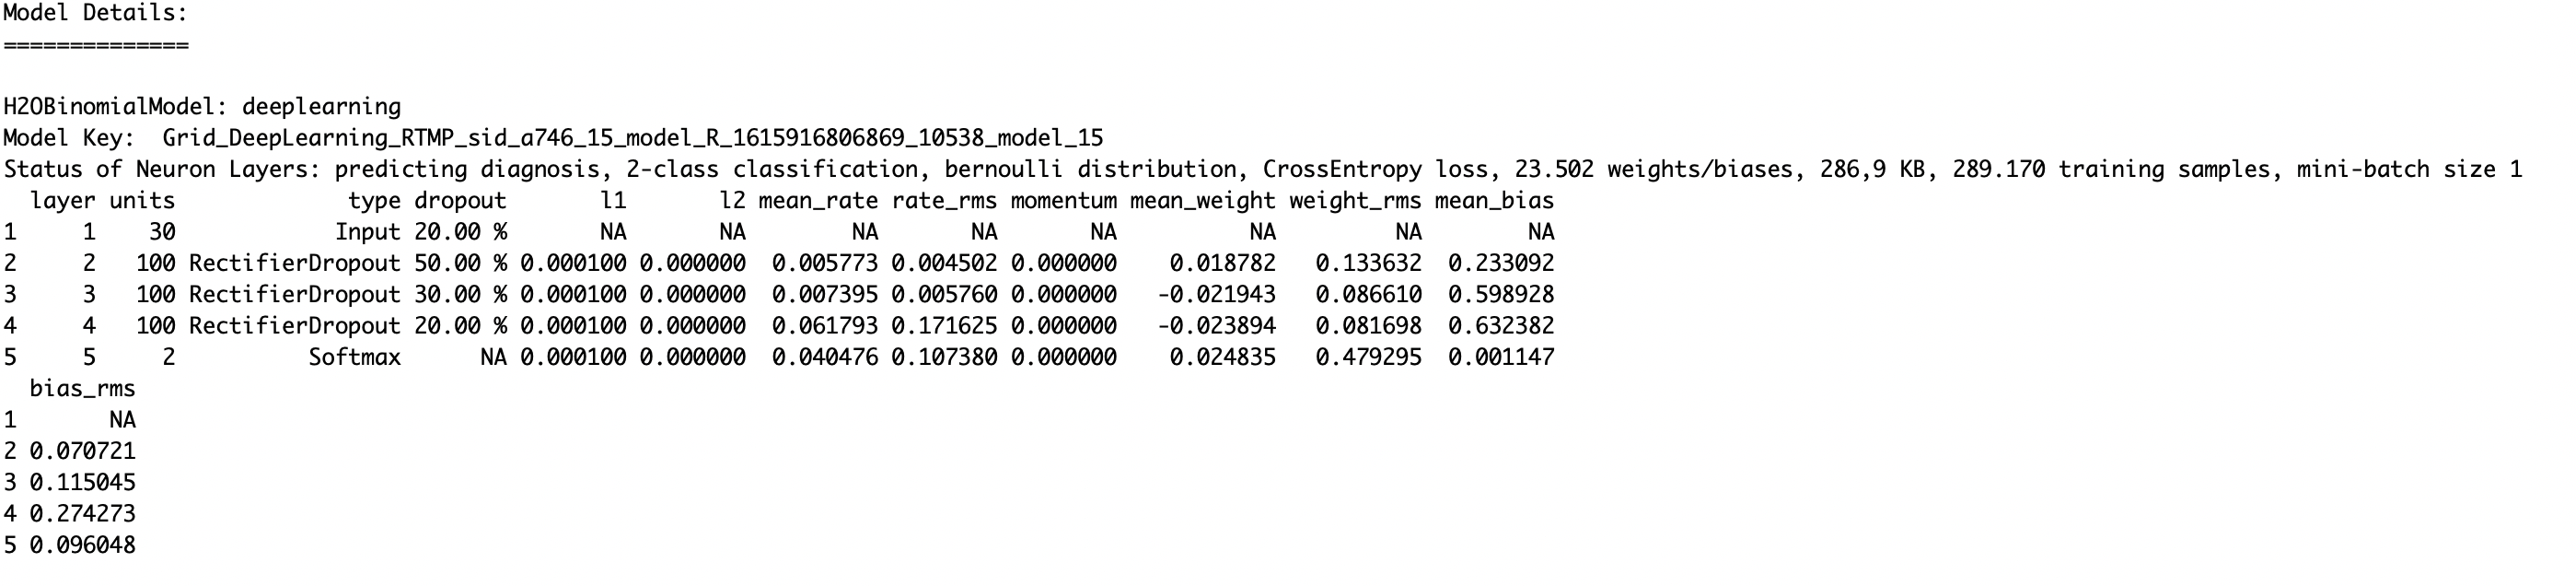
\includegraphics[width=1\textwidth]{images/model_details.png}
    \caption{Summary of the choosen Artificial Neural Network}
    \label{fig:model_details}
\end{figure}

\begin{figure}
    \centering
    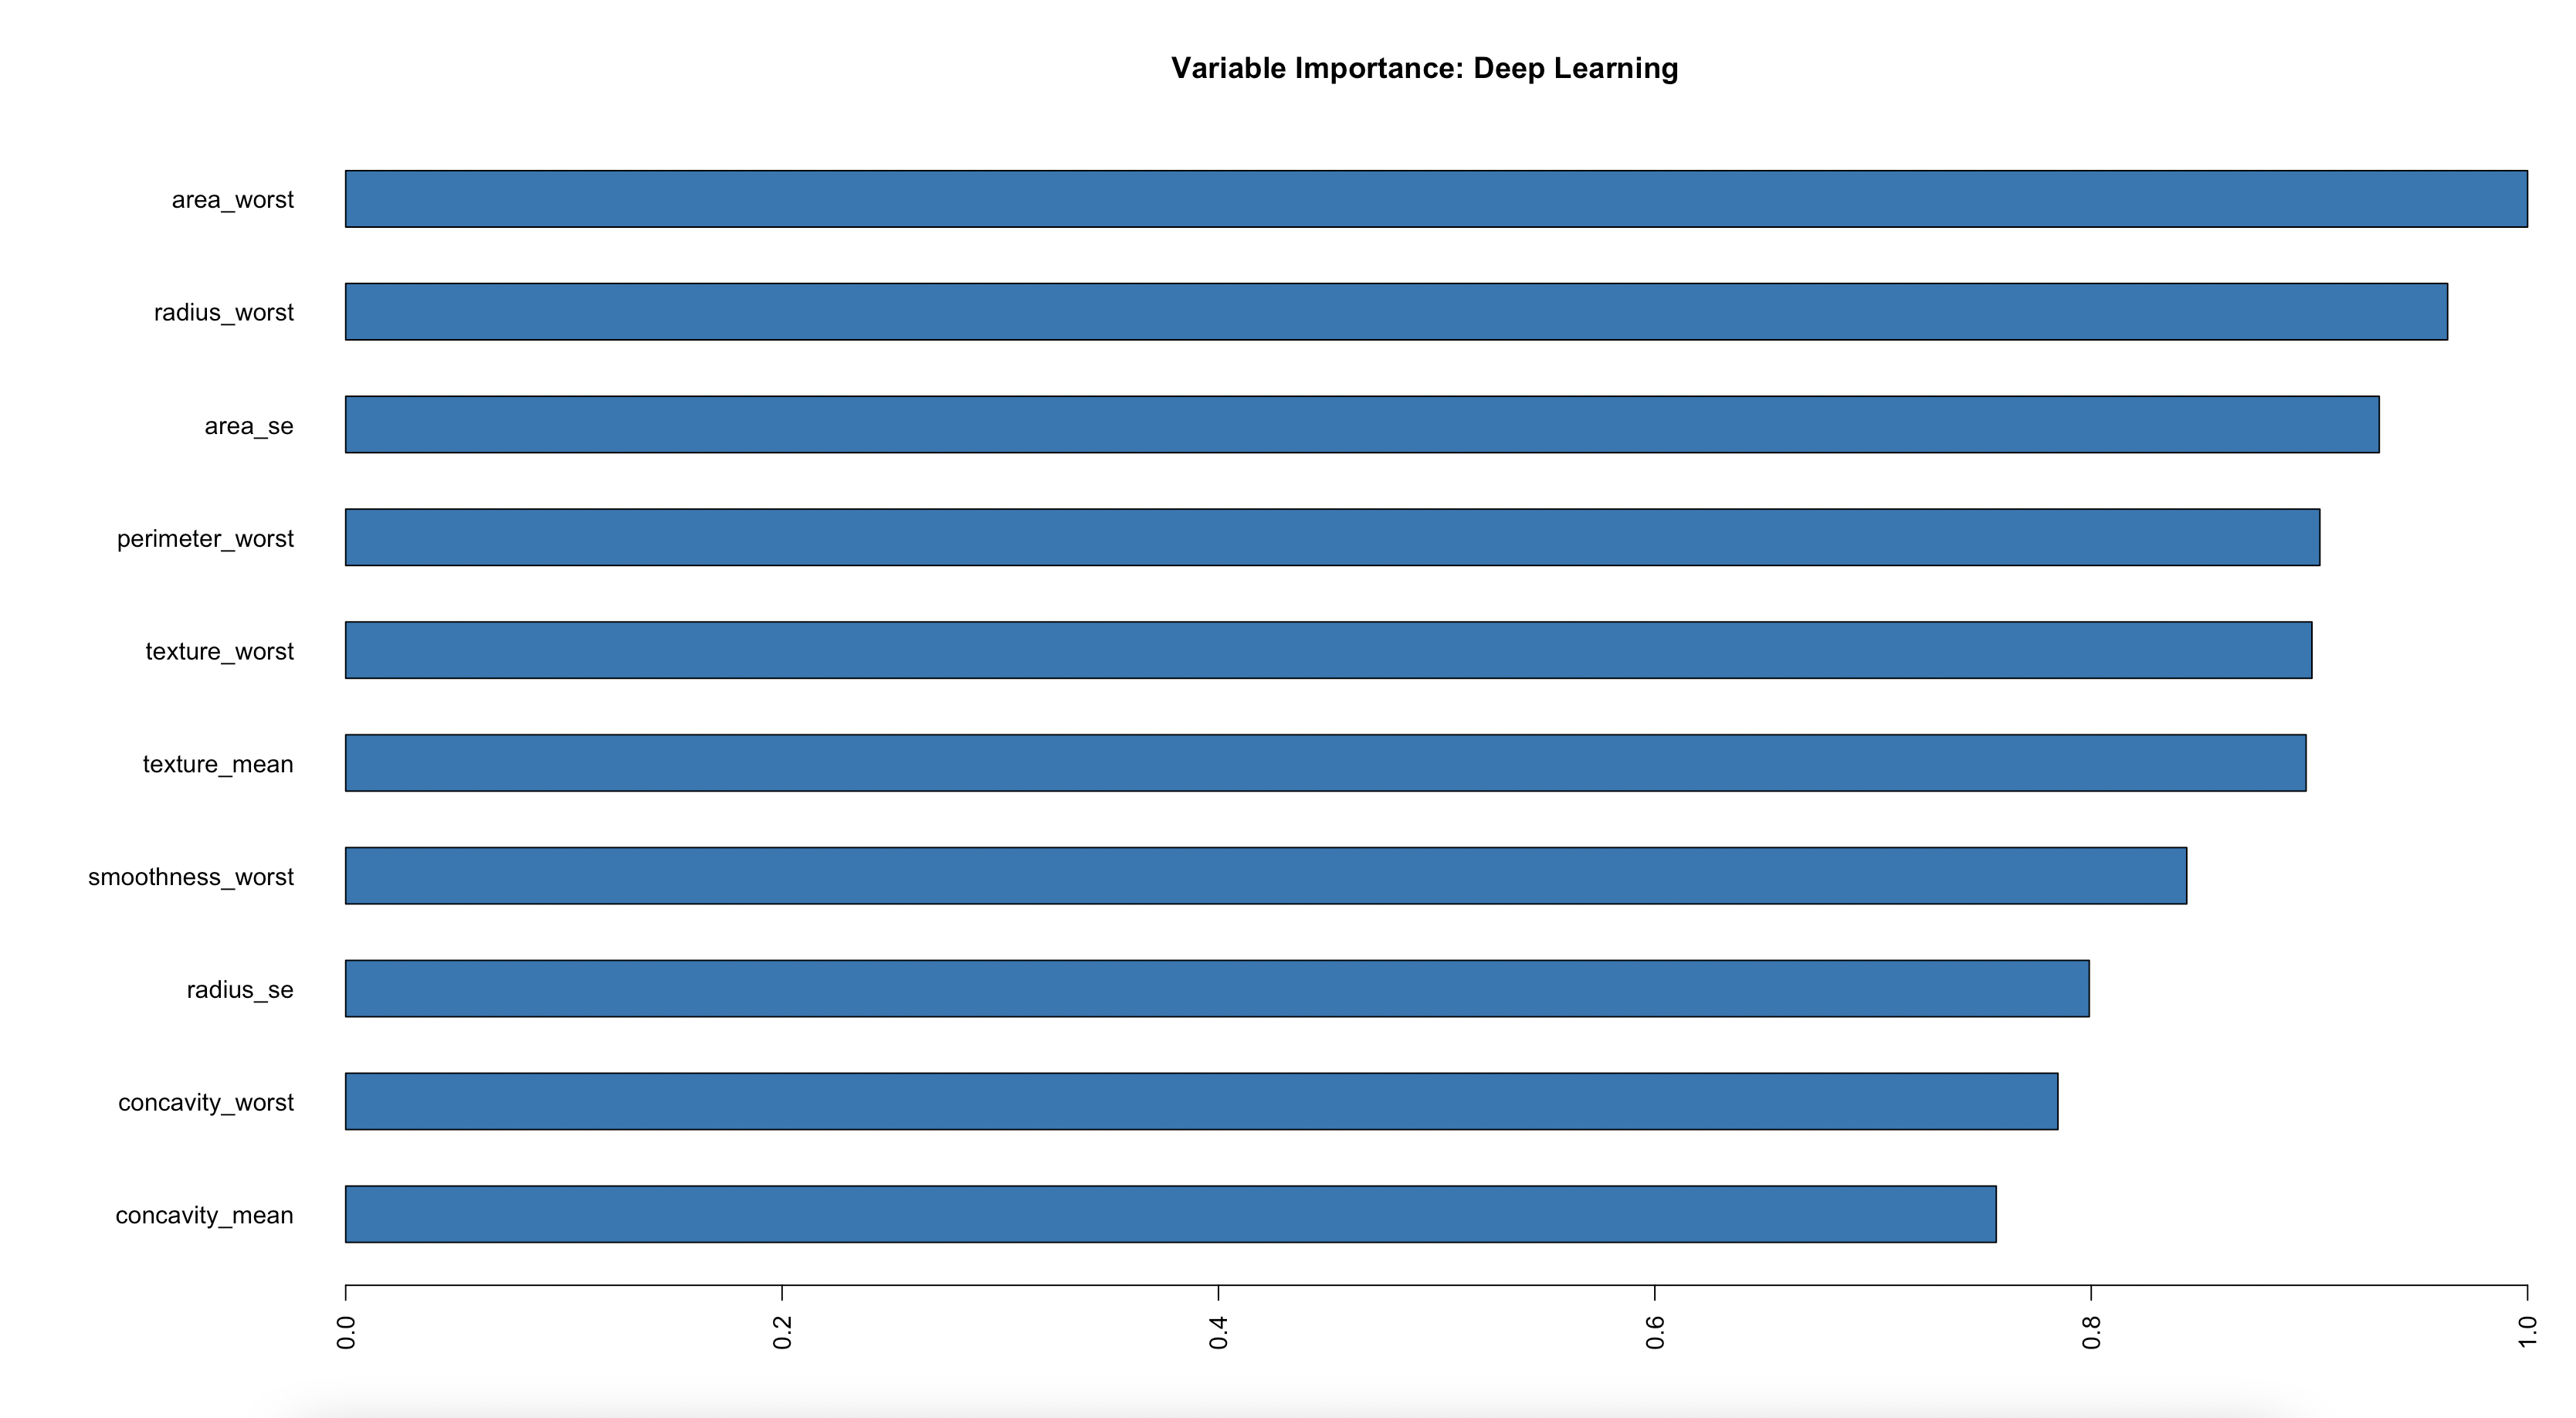
\includegraphics[width=0.8\textwidth]{images/variable_importance.png}
    \caption{Variable Importance of the choosen Artificial Neural Network}
    \label{fig:variable_importance}
\end{figure}

\subsubsection{Criteria}\label{criteria}

\paragraph{Explainibility}\label{explainibility}

We did choose the R-Package h2o over nnet for it's great explainability.

\paragraph{Expert Plots}\label{expert-plots}

A deeper understanding of a fittet model can be gained with a variety of
plots. For an ANN a Partial Dependence Plot or the Individual
Conditional Expectation Plot of a given column can be visualized.

\begin{figure}
    \centering
    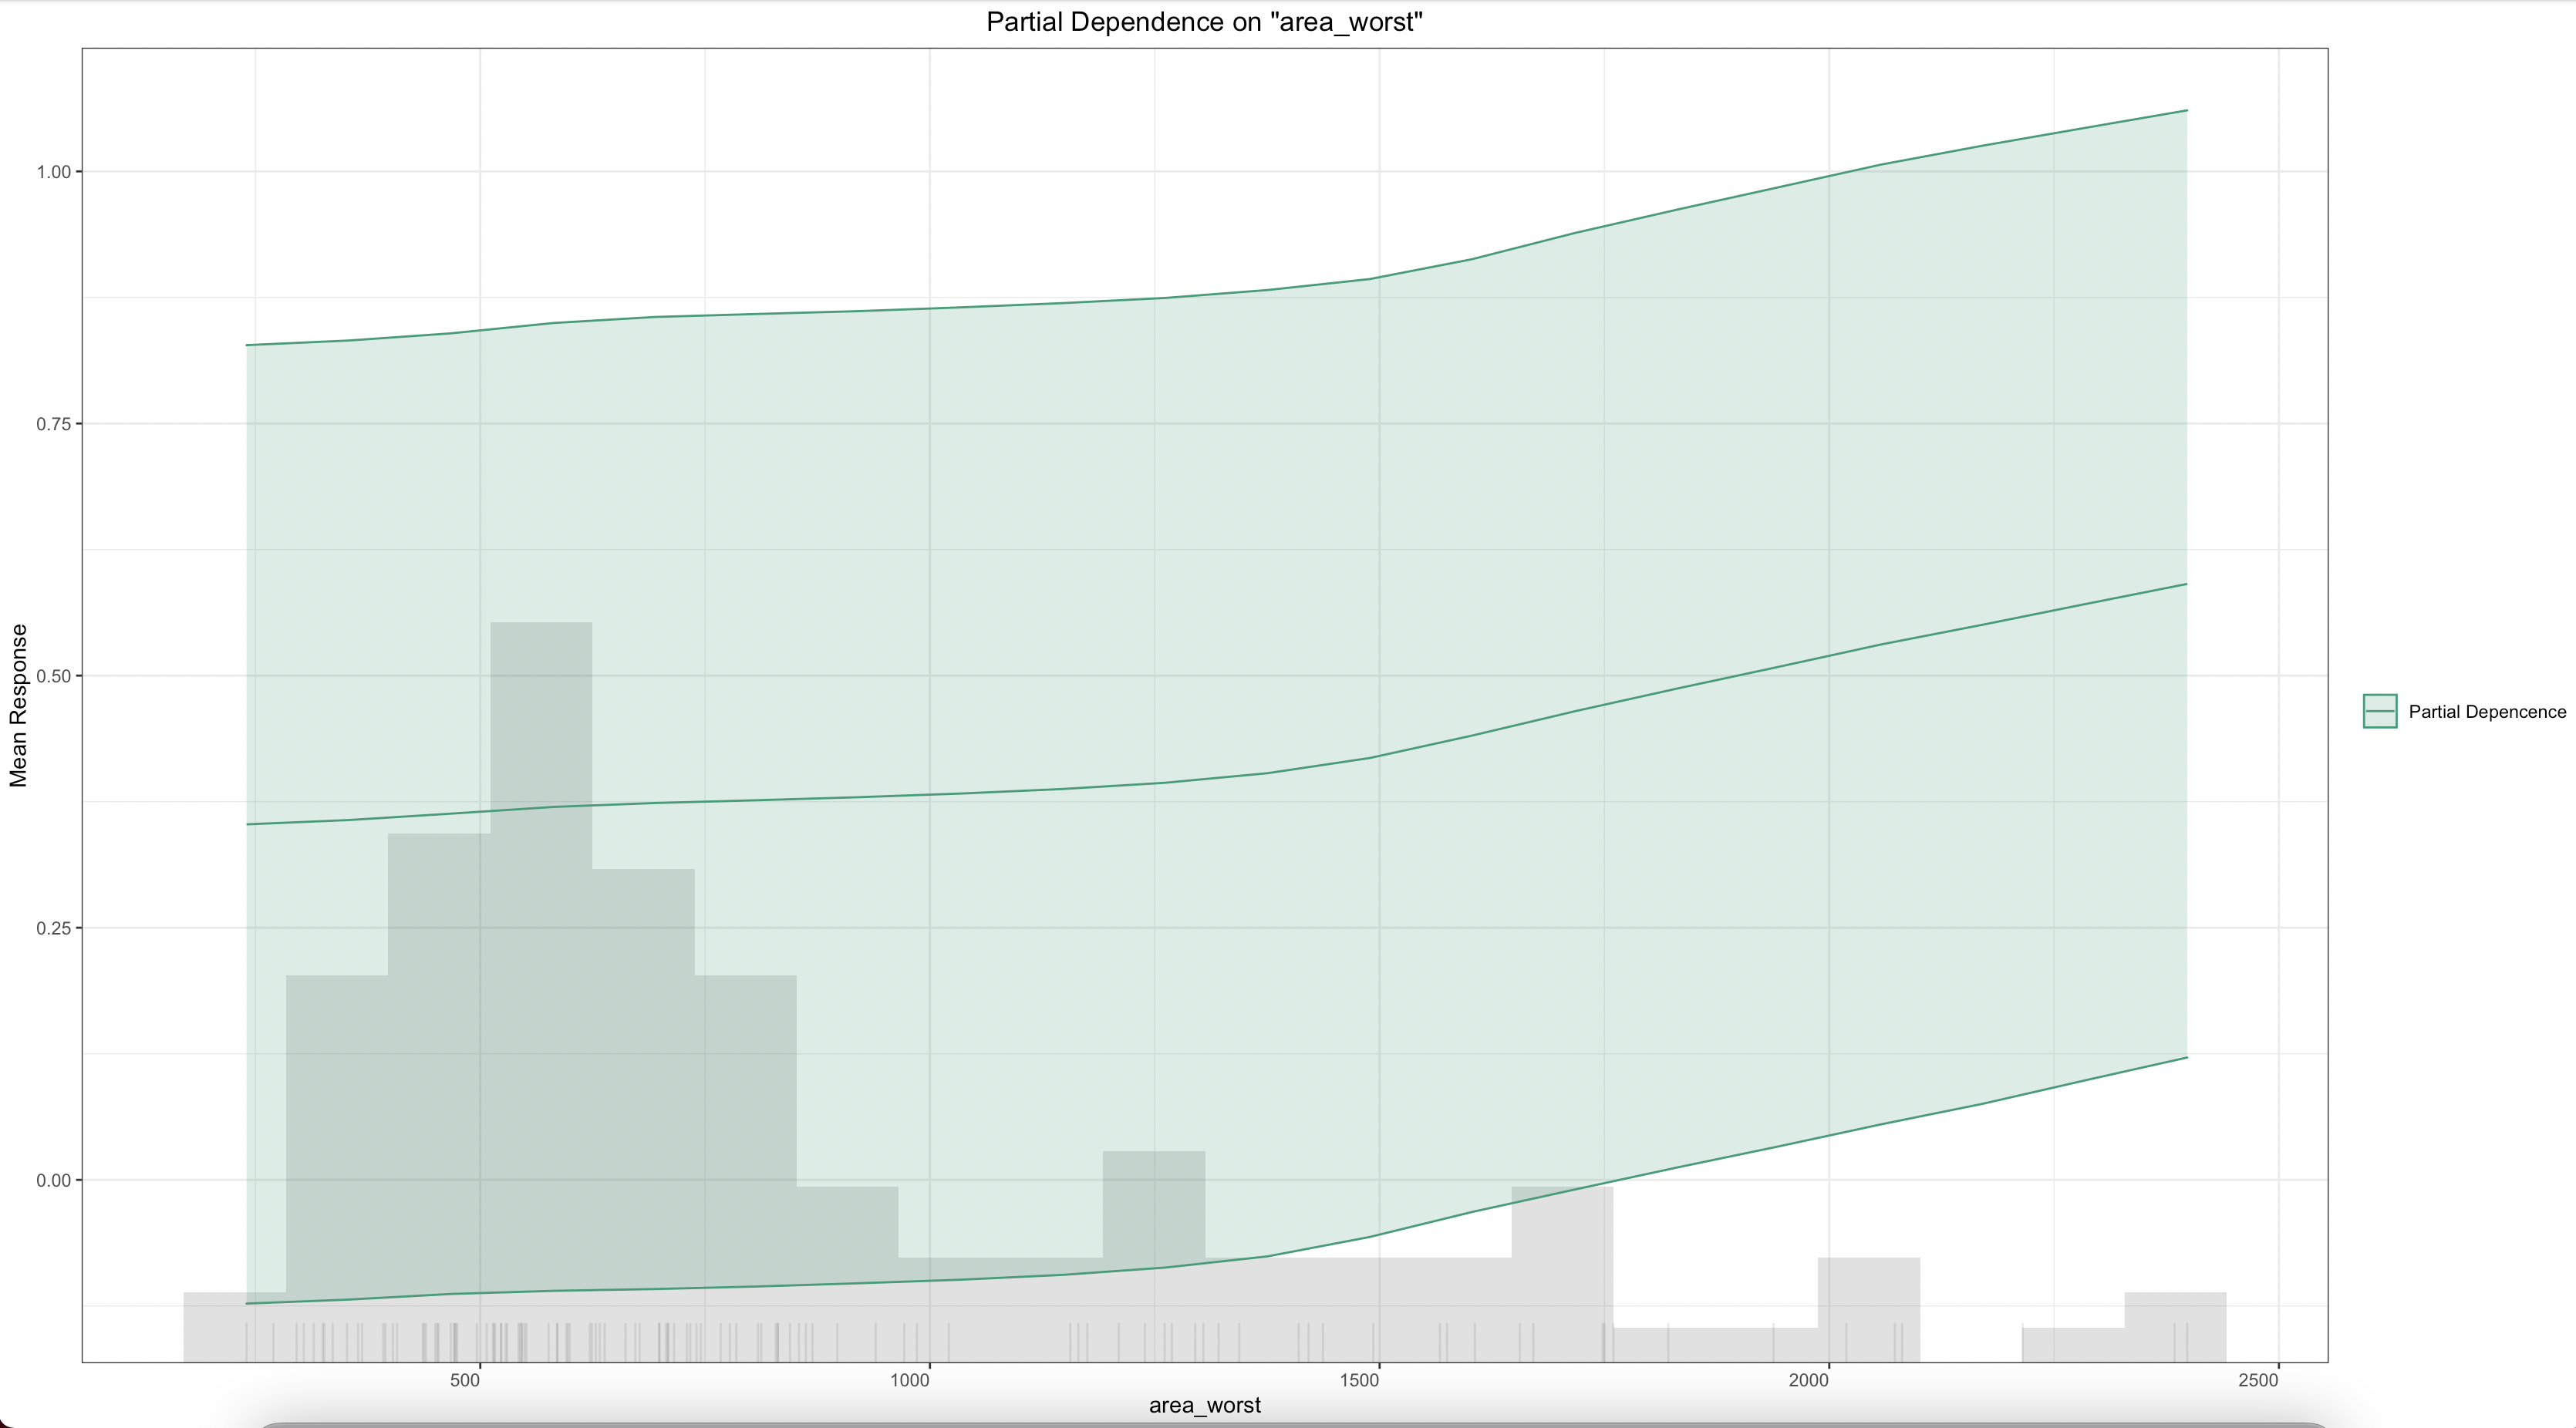
\includegraphics[width=0.8\textwidth]{images/pd_plot.png}
    \caption{Partial Dependence Plot wrt area\_worts}
    \label{fig:pd_plot}
\end{figure}

\begin{figure}
    \centering
    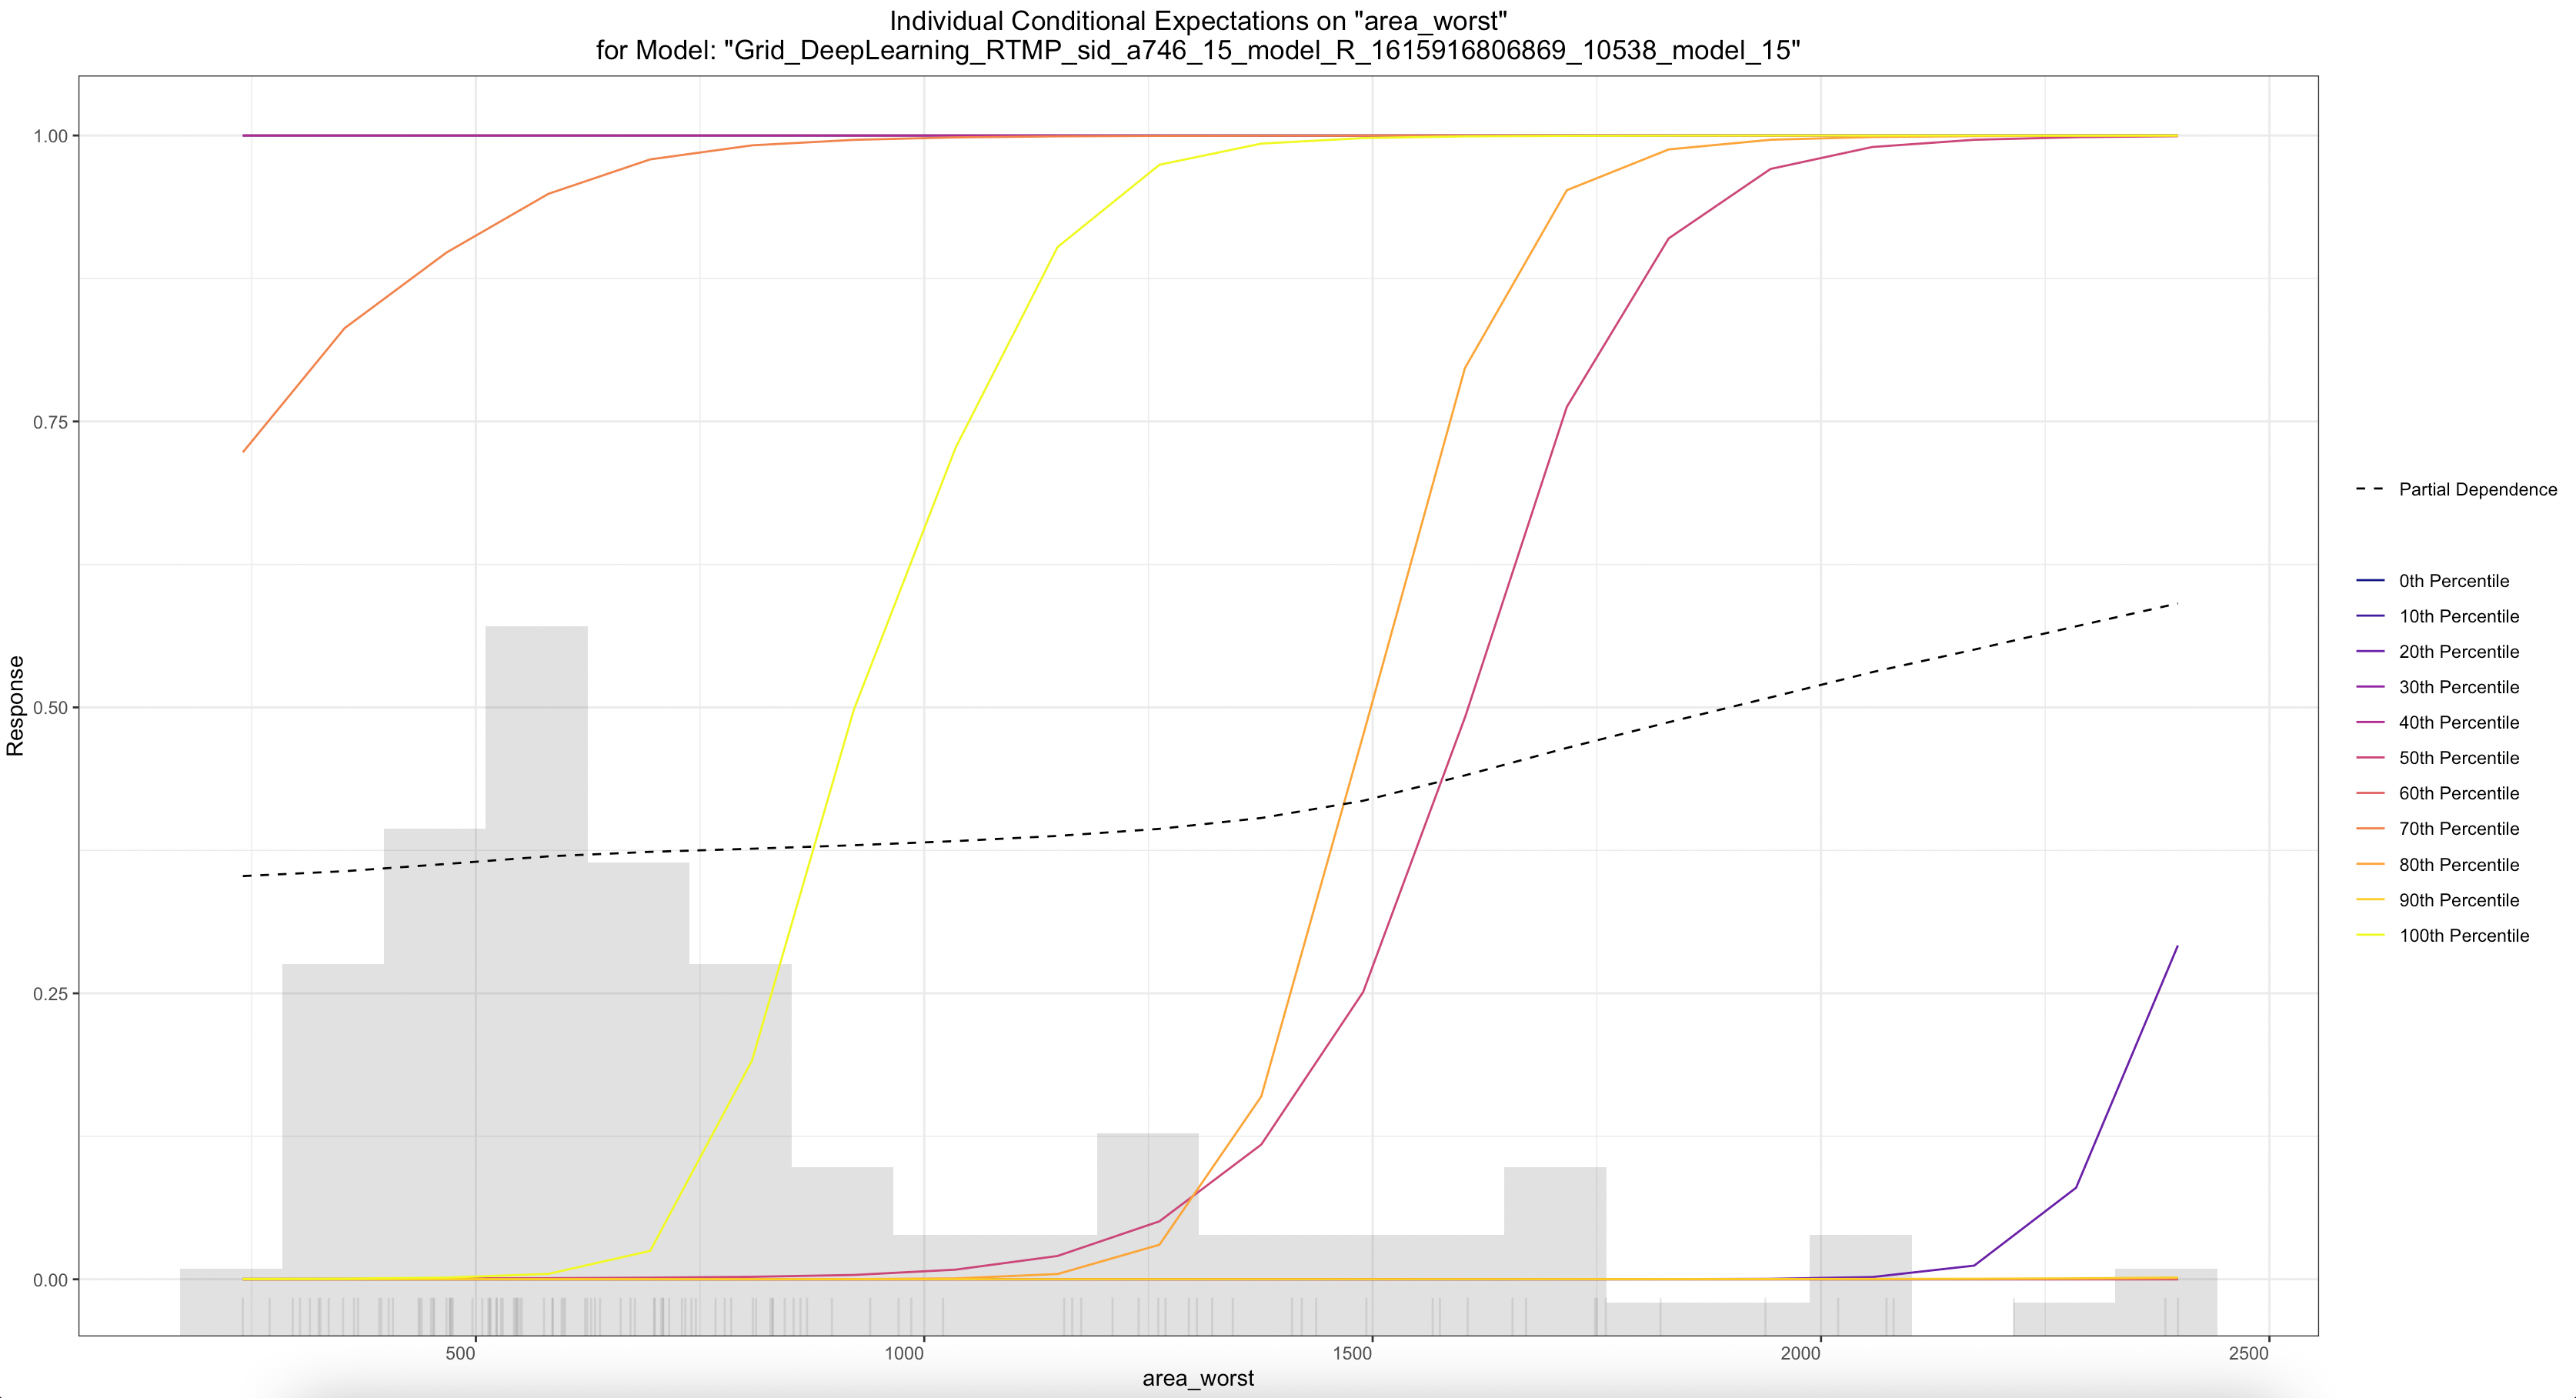
\includegraphics[width=0.8\textwidth]{images/ice_plot.png}
    \caption{Conditional Expectation Plot wrt area\_worst}
    \label{fig:ice_plot}
\end{figure}

\section{Final Assessment}\label{final-assessment}

We compare the logistic regression and the neural networks wrt accuracy
and sensitivity and specificity on the test set.

\begin{center}
 \begin{tabular}{|c | c |  c | c|} 
 \hline
 Model & Accuracy & Sensitivity/Recall & Specificity \\ [0.5ex] 
 \hline
 Logistic regression & .95 & .95 & .95 \\ 
 \hline
 Neural Network & .98 & 1 & 1 \\
 \hline
\end{tabular}
\end{center}

The neural network performs better in every criterion.

We should show AUC for both methods?!

\begin{figure}
    \centering
    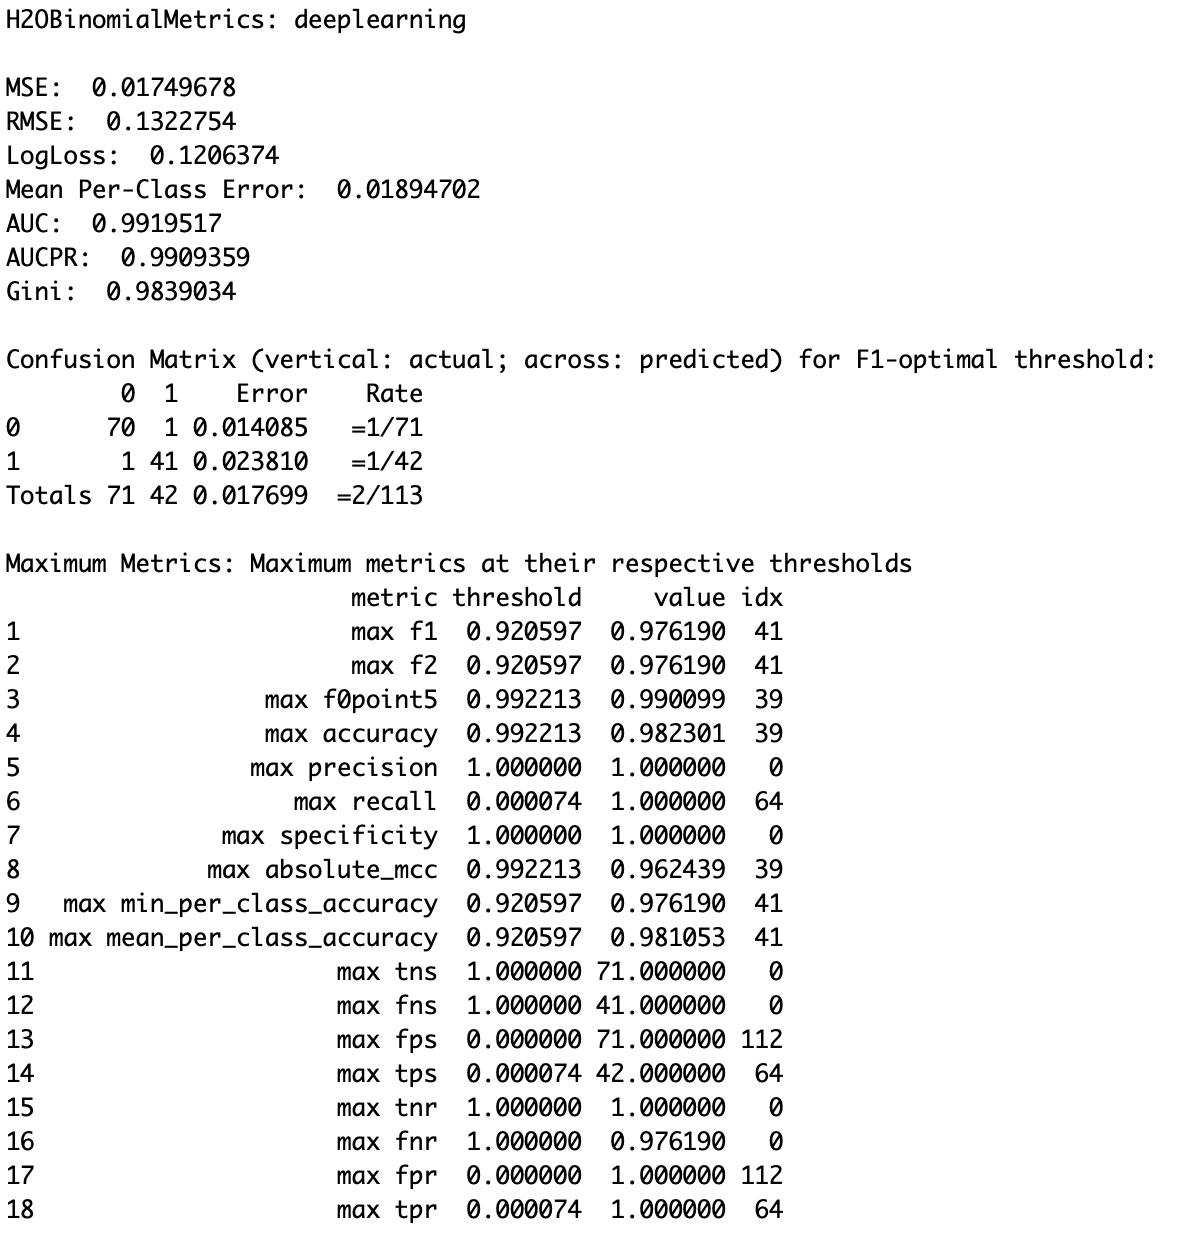
\includegraphics[width=0.8\textwidth]{images/h2o_model_performance.png}
    \caption{Metrices of the choosen Artificial Neural Network}
    \label{fig:h2o_model_performance}
\end{figure}

please, see the notebook for more details.

\section{Deployment}\label{deployment}

Something on meeting the standards to deploy an algorithm in medical
diagnosis. Who decides? What are the criteria.

\section{How to insert References}\label{how-to-insert-references}

\cite{nnet}

\cite{otexts}

\section{Figures I wasn'T sure were to
insert}\label{figures-i-wasnt-sure-were-to-insert}

\begin{figure}
    \centering
    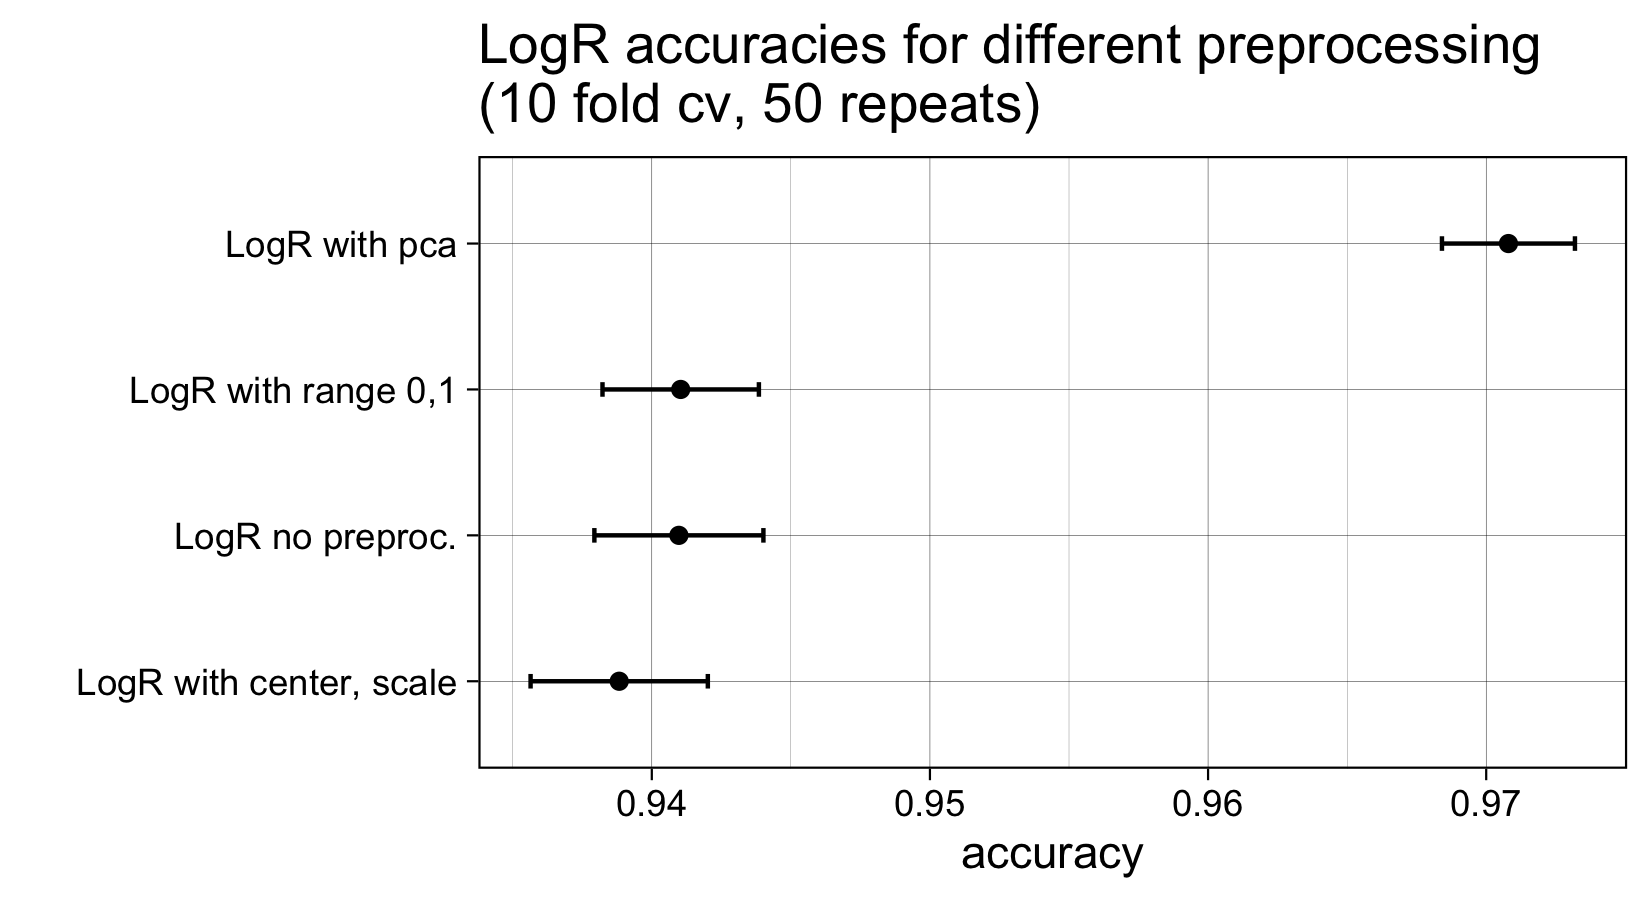
\includegraphics[width=0.8\textwidth]{images/M1-preprocessing-options.png}
    \caption{Preprocessing Options}
    \label{fig:preprocessing}
\end{figure}

\begin{figure}
    \centering
    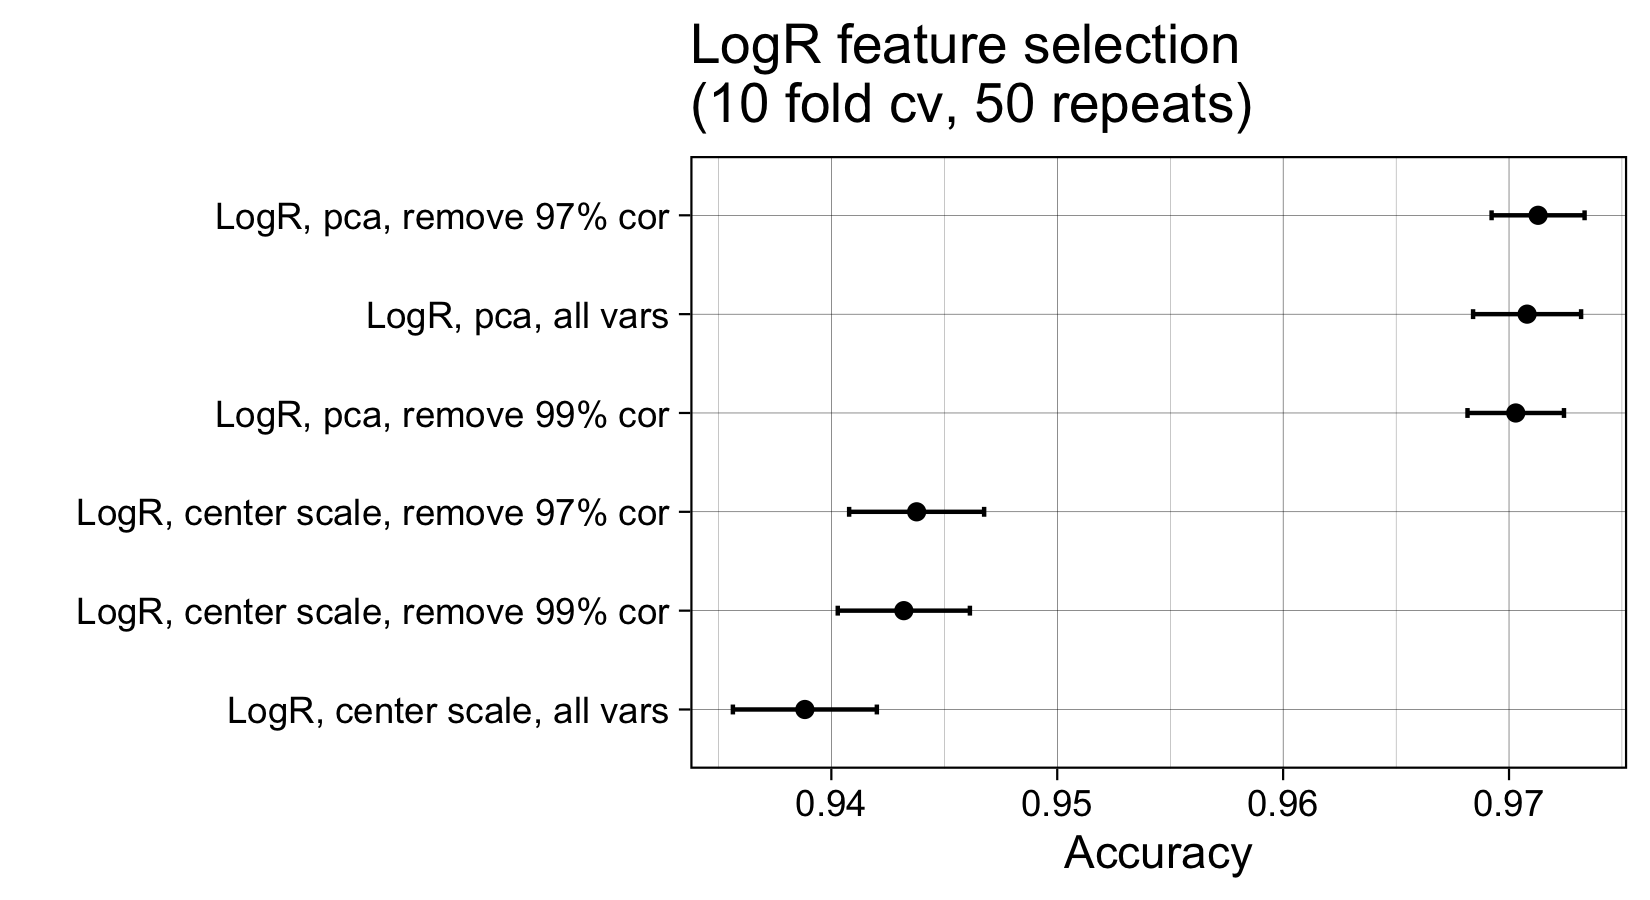
\includegraphics[width=0.8\textwidth]{images/M2-feature-selection.png}
    \caption{Feature Selection}
    \label{fig:feature-selection}
\end{figure}

\renewcommand\refname{References}
\bibliography{references.bib}

\end{document}
